\section{Τεχνολογίες που χρησιμοποιήθηκαν}
\label{section:tools}

Στην τελευταία υποενότητα αυτού του κεφαλαίου θα μιλήσουμε για τα εργαλεία που χρησιμοποιήθηκαν
για την υλοποίηση του συστήματος Αυτόματης Παρακολούθησης που υλοποιήσαμε στο πλαίσιο της διπλωματικής
αυτής εργασίας.

\subsection{Node.js}
\label{subsec:nodejs}

Είναι ένα περιβάλλον εκτέλεσης (runtime) της προγραμματιστικής γλώσσας JavaScript.
Πληθώρα μηχανικών λογισμικού το χρησιμοποιούνε σήμερα, για τη γρήγορη και, σχετικά με άλλα εργαλεία,
εύκολη ανάπτυξη διαδικτυακών εφαρμογών. Η Node.js μάλιστα διαθέτει το δικό της package manager
(ΝPM - Node Package Manager), στον οποίο διαρκώς προστίθενται καινούργιες βιβλιοθήκες
από χρήστες για χρήστες. 

Είναι σχεδιασμένο για να μπορεί να χτίζει κλιμακούμενες (scalable) εφαρμογές, καθώς η αρχιτεκτονική του,
επιτρέπει τη σύνδεση πολλών εξωτερικών συστημάτων/χρηστών και την εξυπηρέτηση αυτών ταυτόχρονα. Κάθε φορά που γίνεται κάποια σύνδεση στην εφαρμογή εκτελείται μία callback συνάρτηση προκειμένου να μπορέσει να απαντήσει πίσω.
Όσο το σύστημα δεν δέχεται αιτήματα "κοιμάται" και περιμένει το επόμενο που θα έρθει.

Όλα όσα προαναφέρθηκαν την καθιστούν κατάλληλη για τη δημιουργία συστημάτων server. Αξίζει να σημειωθεί μάλιστα ότι για το σκοπό
αυτό υπάρχουν πλήθος βιβλιοθηκών που παρέχουν έτοιμες συναρτήσεις και διεπαφές που κάνουν την διαδικασία ανάπτυξης ακόμα πιο εύκολη
και γρήγορη. Πολλές φορές μάλιστα, κάποιες βιβλιοθήκες πέρα από βοηθητικές συναρτήσεις και υπορουτίνες, επηρεάζουν τον τρόπο
συγγραφής κώδικα, μέσα από APIs που παρέχουν. Αυτές χαρακτηρίζονται ως frameworks, και επιταχύνουν τόσο τη διαδικασία
ελέγχου (testing), όσο και τη διαδικασία ανάπτυξης (development) του λογισμικού. Μερικά από τα πιο γνωστά
backend framerworks είναι τα: Express, Jest, Koa, Socket.io, Meteor, Loopback

Τα παραπάνω, σε συνδυασμό με το ότι η JavaScript είναι μία ευρέως διαδεδομένη και πολυχρησιμοποιούμενη γλώσσα
προγραμματισμού στο διαδίκτυο, δίνει την ευκαιρία σε developers να αναπτύξουν μία εφαρμογή πλήρως
(frontend και backend) με τη χρήση ενός κοινού εργαλείου. Ένα τυπικό παράδειγμα εφαρμογής που μπορεί να
αναπτυχθεί με τον τρόπο αυτό φαίνεται στο \autoref{fig:nodejs_system}.

\begin{figure}[!ht]
	\centering
	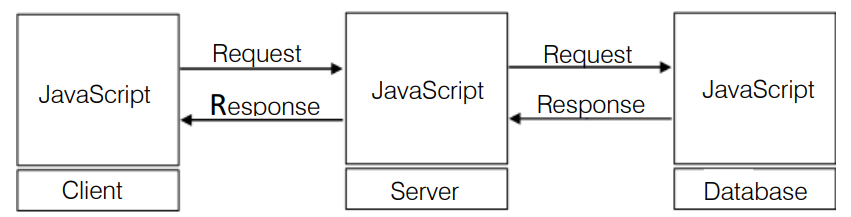
\includegraphics[width=0.8\textwidth]{./images/chapter2/javascript_end_to_end.png}
	\caption[Σχεδίαση συστήματος με χρήση Node.js]{Σχεδίαση συστήματος με χρήση Node.js \cite{nodejs_challenges_in_implementation}}
	\label{fig:nodejs_system}
\end{figure}

\subsection{PM2}
\label{subsec:pm2}

Η διαχείρηση διεργασιών (processes) που τρέχουν σε ένα υπολογιστικό σύστημα μπορεί να είναι δύσκολη
και αρκετά περίπλοκη για κάποιον που δεν διαθέτει μεγάλη πείρα σε αυτό τον τομέα. Το PM2, ή αλλιώς Process Manager 2,
αποτελεί ένα έργο λογισμικού ανοιχτού κώδικα (open source project), που κάνει την παραπάνω διαδικασία πιο απλή και κατανοητή, κερδίζοντας χρόνο
για τον developer που μπορεί να τον αξιοποιήσει για την ανάπτυξη εφαρμογών.

Με την έννοια διαχείρηση διεργασιών, αναφερόμαστε σε όλες εκείνες τις ενέργειες που σχετίζονται
με τον (πρόωρο ή όχι) τερματισμό και την παρακολούθηση ήδη υπάρχοντων διεργασιών (\autoref{fig:pm2_monitoring}), αλλά και τη δημιουργία καινούργιων.
Προγράμματα όπως το pm2 προσφέρουν ακόμα δυνατότητες όπως είναι η αυτόματη επανεκκίνηση διεργασιών σε περίπτωση σφάλματος
αποτρέποντας έτσι την ύπαρξη downtime των εφαρμογών που τρέχουμε.

Ένα από τα πιο χρήσιμα εργαλεία που παρέχει το PM2 είναι η λειτουργία cluster mode.
Αν και δεν αναφέρθηκε πιο πάνω, ο συγκεκριμένος διαχειριστής διεργασιών εξειδικεύεται σε Node.js
εφαρμογές και στη διαχείρηση αυτών. Εξ ορισμού, εφαρμογές γραμμένες σε JavaScript τρέχουν σε ένα νήμα (thread)
στο υπολογιστικό σύστημα που εκτελούνται. Χρησιμοποιώντας όμως το cluster mode, μπορούμε να
ξεκινήσουμε πολλαπλές διεργασίες που θα λειτουργούν ταυτόχρονα και θα μοιράζουν το φόρτο
κατάλληλα (load-balancing) ώστε το τελικό σύστημα να έχει καλύτερη απόδοση και να μπορεί να εξυπηρετεί 
περισσότερο κόσμο. 

\begin{figure}[!ht]
	\centering
	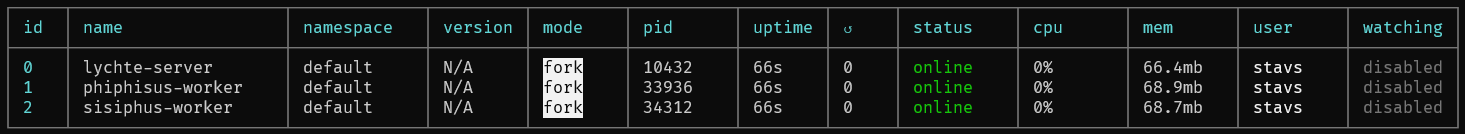
\includegraphics[width=1\textwidth]{./images/chapter2/pm2_monitoring.png}
	\caption[Παράδειγμα Παρακολούθησης διεργασιών με τη χρήση του PM2]{Παράδειγμα Παρακολούθησης διεργασιών με τη χρήση του PM2}
	\label{fig:pm2_monitoring}
\end{figure}

\subsection{MongoDB}
\label{subsec:mongodb}

H MongoDB αποτελεί μία Μη Σχεσιακή Βάση Δεδομένων (Non Relational Data\hyp{}base), που χρησιμοποιεί documents,
για να αποθηκεύσει πληροφορία, αντί στήλες και γραμμές όπως θα είχαμε σε κλασσικές SQL βάσεις δεδομένων.
Είναι σχεδιασμένη για αποθήκευση δεδομένων μεγάλης κλίμακας και παράλληλη επεξεργασία δεδομένων μοιρασμένα
σε έναν μεγάλο αριθμό από servers. 

Τα documents που αναφέρθηκαν αποτελούν τον ακρογωνιαίο λίθο της Mongo, καθώς αποτελούν τη βασική μονάδα
της αποθηκευμένης πληροφορίας. Μορφοποιούνται ως BJSON (Binary JSON) και παρέχουν πληθώρα τύπων δεδομένων
που μπορούν να αποθηκευτούν (string, integer, double, boolean, array, object, date, time\hyp{}stamp, null, binary). Κάθε βάση mongo μπορεί να περιέχει μία ή περισσότερες συλλογές (collections),
τα δεδομένα των οποίων πρέπει να υπακούουν στο ίδιο σχήμα (schema). Επειδή όμως η βάση αυτή παρέχει
δυνατότητες δυναμικού σχήματος (dynamic schema) μπορούμε να αποθηκεύουμε πληροφορία και να προσθέτουμε πεδία (fields)
που δεν είχαμε ορίσει από την αρχή δημιουργίας του συστήματος. \\

Μερικοί από τους λόγους που την επιλέξαμε είναι οι εξής:

\begin{itemize}
	\item \textbf{Document Oriented Storage}: η αποθήκευση και διαχείριση των δεδομένων
		(στο πλαίσιο της εφαρμογής) είναι εύκολη καθώς στηρίζεται σε δεδομένα σε μορφή JSON.
	\item \textbf{Ευρετήρια (Indexes)}: Υπάρχει η δυνατότητα, κατά τη διαδικασία του στησίματος της βάσης (αλλά και μετέπειτα),
		να οριστούν ευρετήρια σε πεδία που χρησιμοποιούνται συχνά σε queries, προκειμένου
		να βελτιωθεί η απόδοση του συστήματος στο σύνολο. Όσο πιο γρήγορη είναι βάση, τόσο
		καλύτερη θα είναι η ανταπόκριση του συστήματος. 
	\item \textbf{Ομοιοτυπία (Replication) και μεγάλη Διαθεσιμότητα}: Δημιουργώντας πολλαπλά αντίτυπα των αποθηκευμένων δεδομένων	
		σε περισσότερους από έναν servers, μπορούμε να είμαστε σίγουροι ότι θα έχουμε πρόσβαση στην
		πληροφορία ακόμα και αν η κίνηση (data traffic) της εφαρμογής αυξηθεί.
	\item \textbf{Αυτόματο sharding}: Διασπώντας την αποθηκευμένη πληροφορία και έχοντας τμήματα αυτής σε διαφορετικούς server
		μας δίνεται η δυνατότητα να κάνουμε οριζόντιο scaling πολύ πιο εύκολα. 
	\item \textbf{Εύκολη ενσωμάτωση}: Η mongo διαθέτει βιβλιοθήκες στο περιβάλλον του node.js που καθιστούν
		τη χρήση και το στήσιμό της πολύ απλά. Πέρα από τη mongo, την επίσημη βιβλιοθήκη που υπάρχει,
		διατίθεται και η mongoose που αποτελεί μία Object Data Modelling (ODM) βιβλιοθήκη για τη Mongo και τη nodejs (\autoref{fig:mongoose}) 
\end{itemize}
\begin{figure}[H]
	\centering
	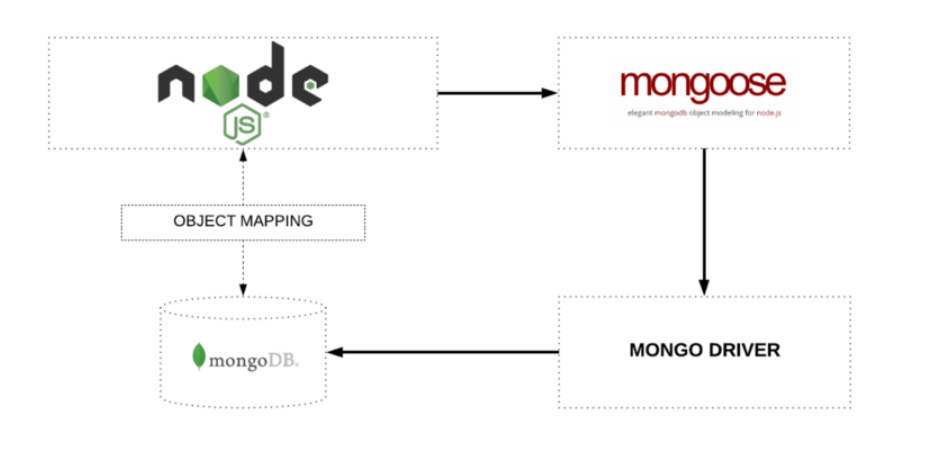
\includegraphics[width=0.8\textwidth]{./images/chapter2/mongoose.png}
	\caption[Mongoose, ένα abstract layer μεταξύ Node και mongo]
	{H mongoose λειτουργεί ώς ένα abstract layer μεταξύ της Node και των driver της mongo προκειμένου η επικοινωνία μεταξύ των δύο να γίνεται πιο εύκολα}
	\label{fig:mongoose}
\end{figure}

\vfill
\break

\subsection{Google Cloud Storage}
\label{subsec:gcloud}

Πέρα από την κλασική βάση δεδομένων που προαναφέρθηκε θέλουμε να αποθηκεύουμε ιστορικά δεδομένα,
δεδομένα δηλαδή που δεν θα εμφανίζονται άμεσα στον χρήστη, αλλά θα χρησιμοποιούνται για τον υπολογισμό μετρικών και στατιστικά σημαντικών αποτελεσμάτων,
στο σύνολο όλης της μέχρι τώρα αποθηκευμένης πληροφορίας.

Σε αυτό λοιπόν το σημείο έρχεται το Google Cloud Storage (GCS), το οποίο παρέχει μεταξύ άλλων, δυνατότητες
Αποθήκευσης Αρχείων (File Storage). Τα δεδομένα αυτά δεν χρειάζεται να υπακούουν σε κάποιο σχήμα,
ενώ παράλληλα ο τρόπος αρχειοθέτησης των δεδομένων ταυτίζεται με ένα κλασικό σύστημα αρχείων
ενός υπολογιστικού συστήματος. Διαθέτει paths και τύπους αρχείων όπως ακριβώς και οι υπολογιστές και όλες οι
συσκευές που χρησιμοποιούμε. Για να διαβάσει κανείς πληροφορία, χρειάζεται να ξέρει μόνο το μονοπάτι που οδηγεί
στο επιθυμητό αρχείο, καθώς και τη μορφή αυτού. Οι υποστηριζόμενοι τύποι αρχείων μέχρι τώρα είναι οι εξής:

\begin{itemize}
	\item Binary
	\item Flat
	\item JSON
	\item Avro
	\item Parquet
\end{itemize}

\subsection{Rust Language}
\label{subsec:rust}
Η Rust αναδεικνύεται ως μια σύγχρονη γλώσσα προγραμματισμού που έχει κερδίσει δημοτικότητα για την ασφαλή και αποτελεσματική ανάπτυξη συστημάτων. Η Rust παρέχει ένα πλαίσιο που ενσωματώνει σημαντικές έννοιες για τη δημιουργία αξιόπιστου και αποτελεσματικού κώδικα.

Παρακάτω αναπτύσσονται οι βασικές έννοιες της Rust:

\begin{itemize}
\item Ownership: Η Rust χρησιμοποιεί ένα σύστημα ιδιοκτησίας για τη διαχείριση της μνήμης. Αυτό σημαίνει ότι κάθε κομμάτι δεδομένων έχει έναν "ιδιοκτήτη", που είναι υπεύθυνος για την απελευθέρωση της μνήμης όταν δεν χρειάζεται πλέον \cite{rust2}.
\item Borrowing: Μηχανισμός κατά τον οποία τμήματα δεδομένων δανείζονται στιγμιαία σε άλλο σημειο του κώδικα χωρίς να μεταφέρεται το ownership \cite{rust1}. Με τον τρόπο αυτό, μειώνεται η ανάγκη παρουσίας πολλών αντιγράφων των δεδομένων σε διαφορετικά σημεία του κώδικα. Ο δανεισμός δεδομένων πραγματοποιείται σε 2 σημεία. Τα mutable borrows αναφέρονται σε πρόσβαση με δικαιώματα read και write. Τα immutable αναφέρονται σε πρόσβαση με δικαιώματα read.
\item Lifetimes: Οι διάρκειες ζωής καθορίζουν το χρονικό διάστημα κατά το οποίο είναι έγκυρες οι αναφορές (references) των δεδομένων \cite{rust2}. Αυτό βοηθά στην αποφυγή dangling references (αναφορές προς μνήμη που έχει ήδη απελευθερωθεί) και εξασφαλίζει τη σωστή χρήση των δεδομένων από τις αναφορές.
\end{itemize}

Η Rust υποστηρίζει τη συναρτησιακή προγραμματιστική παραδειγματική, που περιλαμβάνει υψηλή τάξη συναρτήσεων, κλεισίματα (closures), και μονάδες (monads).

\begin{itemize}
\item Closures (Κλεισίματα): Τα κλεισίματα στη Rust είναι σαν ανώνυμες συναρτήσεις που μπορούν να αποθηκευτούν και να περάσουν ως παράμετροι σε άλλες συναρτήσεις. Χρησιμοποιούνται για να δημιουργούνται ευέλικτες λογικές και να αποτρέπουν την ανάγκη για κώδικα πολλαπλών γραμμών.
\item Pattern Matching: Η Rust χρησιμοποιεί το pattern matching για να αντιστοιχίσει τα δεδομένα σε διάφορα πρότυπα, γεγονός που είναι κοινό στη συναρτησιακή προγραμματιστική
\item Iterators (Επαναληπτές): Οι επαναληπτές στη Rust επιτρέπουν τη διατριβή μέσα σε συλλογές δεδομένων με στυλ συναρτησιακού προγραμματισμού.
\end{itemize}

Η προγραμματιστική γλώσσα Rust προσφέρει μια πληθώρα πλεονεκτημάτων:

\begin{itemize}
\item Ασφάλεια Μνήμης: Το σύστημα ιδιοκτησίας (ownership) και ο δανεισμός (borrowing) επιτρέπουν στη Rust να αποφεύγει σχεδόν πλήρως τα σφάλματα μνήμης όπως οι ανεξέλεγκτοι δείκτες και η διαρροή μνήμης. \cite{rust1}.
\item Παράλληλος Προγραμματισμός: Ο παράλληλος προγραμματισμός είναι σχετικά εύκολος στη Rust λόγω του συστήματος ιδιοκτησίας και της ενσωματωμένης υποστήριξης για πολλά νήματα.
\item Χαμηλό Κόστος Αφαιρετικότητας: Η Rust προσφέρει high level abstractions χωρίς να προσθέτει τον επιπλέον χρόνο εκτέλεσης που συνήθως συνοδεύει τις γλώσσες προγραμματισμού με αφαιρετική τυπολογία.Αυτό επιτυγχάνεται με τη χρήση των λειτουργιών:
\begin{itemize}
    \item Zero-cost abstractions: Τα μοτίβα type safety, generics και pattern matching δεν προσθέτουν επιπλέον χρόνο.
    \item No garbage collection: Αυτό επιτυγχάνεται μέσω του συστήματος borrowing και lifetime.
\end{itemize}
\item Performance: Η Rust σχεδιάστηκε για να είναι αποτελεσματική, προσφέροντας χαμηλή ανάλυση και εκτέλεση κοντά στον κώδικα γραμμένο σε C και C++.
\item Κοινότητα και Εργαλεία: Η Rust έχει μια ενεργή κοινότητα και υποστηρίζεται από ένα ισχυρό οικοσύστημα βιβλιοθηκών και εργαλείων ανάπτυξης.
\end{itemize}

\subsection{Python}
\label{subsec:python}

Η Python είναι μια υψηλού επιπέδου γλώσσα προγραμματισμού γνωστή για την απλότητα και την αναγνωσιμότητά της \cite{python1}. Έχει σχεδιαστεί με σκοπό την ευκολία στη κατανόηση και στη συγγραφή, δίνοντας έμφαση στην αναγνωσιμότητα του κώδικα μέσω της χρήσης indentation αντί για αγκύλες ή λέξεις-κλειδιά. H αυτόματη διαχείριση μνήμης της Python ενισχύουν την παραγωγικότητα των προγραμματιστών επιτρέποντας πιο γρήγορους κύκλους ανάπτυξης.

Η απήχηση της Python στην επιστήμη των δεδομένων υποστηρίζεται από το εκτεταμένο εύρος εξειδικευμένων βιβλιοθηκών και frameworks. Κυρίως το NumPy ξεχωρίζει για τον αποτελεσματικό χειρισμό αριθμητικών υπολογισμών, παρέχοντας τη βάση για προηγμένες μαθηματικές πράξεις και χειρισμούς πινάκων \cite{python2}. Συνδυαστικά, η pandas διευκολύνει το χειρισμό και την ανάλυση δεδομένων, προσφέροντας δομές δεδομένων υψηλού επιπέδου. Οι δυνατότητες οπτικοποίησης των δεδομένων ενισχύονται από τα εργαλεία Matplotlib και Seaborn, παρέχοντας τη δυνατότητα για τη δημιουργία περίπλοκων αναπαραστάσεων των δεδομένων \cite{python2}. Αυτά τα εργαλεία είναι καθοριστικά για τη μετάδοση σύνθετων εννοιών και ιδεών. Επιπλέον, η ενσωμάτωση της Python με το Jupyter, ένα διαδραστικό υπολογιστικό περιβάλλον, ενθαρρύνει μια συστηματική και συνεργατική προσέγγιση στην εξερεύνηση και ανάλυση δεδομένων. 

Συγκεκριμένα, στο πεδίο της μηχανικής μάθησης, το scikit-learn είναι μια βιβλιοθήκη για την εφαρμογή αλγορίθμων και στατιστικών μοντέλων. Η σύνταξη της Python είναι συνοπτική στην έκφραση περίπλοκων εννοιών μηχανικής μάθησης, προωθώντας μια βελτιωμένη διαδικασία συλλογιστικής πορείας και ανάπτυξης κώδικα. Επιπλέον, μέσα από την ένταξη της βαθιάς μάθησης δημιουργήθηκαν εργαλεία, όπως το TensorFlow και το PyTorch. Αυτά τα frameworks επιτρέπουν στους ερευνητές να εφαρμόζουν και να πειραματίζονται με αρχιτεκτονικές νευρωνικών δικτύων για δραστηριότητες όπως η ταξινόμηση εικόνων αλλά και η επεξεργασία φυσικής γλώσσας.

Η ευελιξία της Python ενισχύεται από τη διαλειτουργικότητά της με βάσεις δεδομένων, web API και άλλες πηγές δεδομένων. Αυτό το χαρακτηριστικό είναι ιδιαίτερα ωφέλιμο στην επιστήμη δεδομένων, όπου είναι αναγκαίος ο συνδυασμός εργαλείων. Με αυτόν τον τρόπο, επιτρέπει απρόσκοπτες διαδικασίες εξαγωγής, μετασχηματισμού και φόρτωσης δεδομένων (ETL), διευκολύνοντας την ενσωμάτωση διαφορετικών ροών δεδομένων. Η υποστήριξη του RESTful API ενισχύει περαιτέρω τις δυνατότητές της στην πρόσβαση και το χειρισμό δεδομένων από υπηρεσίες web. 

Ο συνεργατικός χαρακτήρας της κοινότητας αποτελεί ένα επιπλέον ωφέλιμο χαρακτηριστικό, το οποίο παρέχει λύσεις, αλλά και ενισχύει ένα περιβάλλον που ευνοεί την ανταλλαγή γνώσης. Επομένως, διασφαλίζονται γρήγορες ενημερώσεις, διορθώσεις σφαλμάτων και εξελίσσονται γοργά τα εργαλεία της επιστήμης δεδομένων για την αντιμετώπιση των αναδυόμενων προκλήσεων.

\subsubsection{Tensorflow}
\label{subsec:tensor}

Το TensorFlow, μια βιβλιοθήκη μηχανικής μάθησης ανοιχτού κώδικα, αντιπροσωπεύει τον ακρογωνιαίο λίθο στη σύγχρονη έρευνα της επιστήμης δεδομένων και της τεχνητής νοημοσύνης. Κεντρικό στοιχείο του σχεδιασμού του είναι η έννοια των υπολογιστικών γραφημάτων, όπου οι λειτουργίες είναι κόμβοι και η ροή δεδομένων αναπαρίσταται μέσω κατευθυνόμενων ακμών. Αυτό το παράδειγμα διευκολύνει αποτελεσματικά τον παράλληλο υπολογισμό, ένα κρίσιμο πλεονέκτημα στις περίπλοκες αρχιτεκτονικές νευρωνικών δικτύων οι οποίες επικρατούν στη σύγχρονη μηχανική μάθηση. 

Η βιβλιοθήκη ασχολείται με τον χειρισμό τανυστών, δηλαδή πολυδιάστατων πινάκων που χρησιμεύουν ως θεμελιώδη δομή δεδομένων. Η ικανότητα του TensorFlow να ενσωματώνεται απρόσκοπτα με το Keras, ένα API νευρωνικών δικτύων υψηλού επιπέδου, παρέχει μια φιλική προς το χρήστη διεπαφή για την κατασκευή και την εκπαίδευση πολύπλοκων μοντέλων, μειώνοντας έτσι το κόστος υλοποίησης \cite{tensorflow2}. 

Η εξέλιξη του TensorFlow στην έκδοση 2.0 εισήγαγε την αυτόματη εκτέλεση, μια αλλαγή από την αρχική προσέγγιση του στατικού γραφήματος. Η αυτόματη εκτέλεση επιτρέπει την άμεση αξιολόγηση των λειτουργιών, βελτιώνοντας τη διαδραστικότητα του κώδικα και απλοποιώντας τη διαδικασία εντοπισμού σφαλμάτων. Επιπλέον, υπάρχει υποστήριξη για κατανεμημένους υπολογιστές, δίνοντας τη δυνατότητα στους χρήστες να αξιοποιήσουν την υπολογιστική ισχύ πολλών CPUs ή GPUs για την εκπαίδευση μοντέλων μεγάλης κλίμακας. Τέλος, κατά την ανάπτυξη, το TensorFlow ενσωματώνει την αρχιτεκτονική του μοντέλου και τα βάρη με τρόπο ανεξάρτητο από την πλατφόρμα. 

Ενισχύεται η διαφάνεια μέσα από το TensorBoard, μια εργαλειοθήκη οπτικοποίησης που διευκολύνει την παρακολούθηση και την απεικόνιση μετρήσεων σε πραγματικό χρόνο κατά τη διάρκεια της εκπαίδευσης των μοντέλων. Τέλος, έχουν δημιουργηθεί διάφορα ακόμη περιβάλλοντα, όπως το TensorFlow Lite για κινητές συσκευές και ενσωματωμένες συσκευές και το TensorFlow.js για τη μηχανική εκμάθηση μέσω προγραμμάτων περιήγησης \cite{tensorflow1}.
        
\subsection{Apache Kafka Queues}
\label{subsec:kafka}

Το Apache Kafka αποτελεί ένα κατανεμημένο σύστημα ανταλλαγής μηνυμάτων που έχει σχεδιαστεί για να αντιμετωπίζει μεγάλο όγκο δεδομένων και να εξασφαλίζει την αντοχή και την απόδοση σε περιβάλλοντα πραγματικού χρόνου \cite{kafka1}.

Τα κύρια χαρακτηριστικά της δομής του συστήματος Kafka είναι:

\begin{itemize}
\item Θέματα (Topics): Τα δεδομένα οργανώνονται σε θέματα, κάθε ένα εκ των οποίων αντιπροσωπεύει μια κατηγορία. Τα μηνύματα στέλνονται σε ένα ειδικό θέμα και διανέμονται σε όλους τους καταναλωτές.
\item Καταναλωτές και Παραγωγοί: Οι παραγωγοί είναι υπεύθυνοι για την αποστολή μηνυμάτων σε ένα θέμα, ενώ οι καταναλωτές λαμβάνουν μηνύματα από τα θέματα και επεξεργάζονται τα δεδομένα.
\item Διαμοιρασμός (Partitioning): Τα θέματα διαιρούνται σε κομμάτια, τα partitions. Αυτό επιτρέπει την κατανεμημένη αποθήκευση και επεξεργασία των δεδομένων.
\end{itemize}

Σχετικά με την λειτουργία του Kafka, σημειώνονται τα παρακάτω στοιχεία λειτουργικότητας:

\begin{itemize}
\item Θέματα (Topics): Αποστολή Δεδομένων (Producer): Ο παραγωγός αποστέλλει μηνύματα σε ένα ή περισσότερα θέματα. Τα μηνύματα είναι ανεξάρτητα και αποθηκεύονται σε partitions.
\item Διανομή Δεδομένων (Brokers): Οι Kafka Brokers αναλαμβάνουν τη διαχείριση των partitions, διανέμοντας τα μηνύματα στους καταναλωτές. Κάθε partition μπορεί να έχει αντίγραφα για αντοχή σε αποτυχία.
\item Λήψη Δεδομένων (Consumer): Οι καταναλωτές εγγράφονται σε ένα ή περισσότερα θέματα και λαμβάνουν τα μηνύματα. Κάθε καταναλωτής είναι υπεύθυνος για το δικό του partition.
\item Συγκράτηση και Διατήρηση Δεδομένων (Retention): Τα μηνύματα διατηρούνται για καθορισμένο χρονικό διάστημα ή μέχρι να φτάσουν σε ένα συγκεκριμένο μέγεθος, εξασφαλίζοντας τη συγκράτηση δεδομένων.
\end{itemize}

Τα μηνύματα αποθηκεύονται με συγκράτηση, διασφαλίζοντας ότι δεν θα χαθούν ακόμη και σε περίπτωση αποτυχίας. Το Kafka είναι εύκολα κλιμακούμενο, διαχειρίζεται υψηλό όγκο δεδομένων και μπορεί να επεκταθεί οριζόντια. Υποστηρίζει τη συμπίεση δεδομένων, βελτιώνοντας την απόδοση και μειώνοντας την κατανάλωση εύρους ζώνης.

Συνολικά, το Apache Kafka αποτελεί ισχυρή λύση για τη διαχείριση ροών δεδομένων σε περιβάλλοντα υψηλής κλίμακας και αξιοπιστίας. Η αρχιτεκτονική του επιτρέπει τη διαχείριση μεγάλων όγκων δεδομένων σε πραγματικό χρόνο \cite{kafka2}. Το Kafka προσφέρει δυνατότητ\vfill
α αποθήκευσης αντιγράφων για εξασφάλιση αντοχής σε αποτυχία. Τα δεδομένα αποθηκεύονται κατανεμημένα σε Brokers, εξασφαλίζοντας ανθεκτικότητα και δυνατότητα εύκολης οριζόντιας επέκτασης.

Το Kafka υποστηρίζει τρία επίπεδα σημασιολογίας: ακριβής, τουλάχιστον ακριβής μία φορά, και ακριβής μία φορά με διατήρηση σειράς. Αυτό επιτρέπει στους παραγωγούς και τους καταναλωτές να επιλέξουν το επίπεδο συνοχής που ταιριάζει με τις απαιτήσεις τους. Επίσης, προσφέρει τα Σημεία Ελέγχου (Checkpoints). Οι καταναλωτές μπορούν να διατηρούν σημεία ελέγχου για το πού έχουν διαβάσει μηνύματα από κάθε partition, εξασφαλίζοντας ότι δεν χάνουν δεδομένα κατά τη διαδικασία επεξεργασίας. Σχετικά με τη διαχείριση απόδοσης, προσφέρεται η Υποστήριξη Συνόλων Ερωτήσεων (Query Sets). Το Kafka Streams API επιτρέπει τη δημιουργία εφαρμογών επεξεργασίας ροών δεδομένων μέσω συνόλων ερωτήσεων, που επιτρέπουν την αναγνώριση των αναγκών επεξεργασίας και ανάκτησης δεδομένων. Τέλος, χρήσιμο εργαλείο αποτελεί η Παρακολούθηση Επίδοσης. Το Kafka παρέχει εργαλεία παρακολούθησης και διαχείρισης, όπως το Kafka Manager, που επιτρέπουν στους διαχειριστές να παρακολουθούν την απόδοση του συστήματος και να λαμβάνουν μέτρα για τυχόν προβλήματα.

\subsection{Docker}
\label{subsec:docker}

Το Docker είναι μια πλατφόρμα ανοιχτού κώδικα που αυτοματοποιεί τη διαδικασία ανάπτυξης, διαχείρισης και εκτέλεσης εφαρμογών σε ελαφριά, φορητά containers. Τα containers παρέχουν ένα συνεχές και απομονωμένο περιβάλλον για την εγκατάσταση εφαρμογών και dependencies, διασφαλίζοντας ότι εκτελούνται με συνέπεια σε διάφορα υπολογιστικά περιβάλλοντα.

Στον πυρήνα του, το Docker χρησιμοποιεί μια αρχιτεκτονική του μοντέλου πελάτη - διακομιστή, όπου ο Docker Daemon διαχειρίζεται containers στο παρασκήνιο και ο Docker Client χρησιμεύει ως διεπαφή. Τα Docker images, τα οποία αποτελούν δομικά στοιχεία των containers, δεν επιτρέπουν την επεξεργασία αλλά μόνο την ανάγνωση και ενσωματώνουν εφαρμογές, βιβλιοθήκες και dependencies, επιτρέποντας την αποτελεσματική κοινή χρήση και διανομή των στοιχείων σε διάφορα περιβάλλοντα \cite{docker2}. Αυτά τα images κατασκευάζονται χρησιμοποιώντας Dockerfiles. Το Dockerfile είναι ένα αρχείο κειμένου που περιέχει οδηγίες για τη δημιουργία ενός Docker image. Καθορίζει το base image, τον κωδικό εφαρμογής, τα dependencies και τη διαμόρφωση.

Τα containers εκτελούν μεμονωμένες διεργασίες, μοιράζονται το kernel του λειτουργικού συστήματος, αλλά διατηρούν ξεχωριστά συστήματα αρχείων και διεργασίες \cite{docker1}. Επιπλέον, υπάρχει το Docker Hub, το οποίο χρησιμεύει ως κοινό αποθετήριο για πρόσβαση σε προκατεσκευασμένα Docker images. Άλλο ένα σημαντικό χαρακτηριστικό είναι τα Docker volumes, τα οποία χρησιμοποιούνται για τη διατήρηση δεδομένων εκτός του συστήματος αρχείων των containers. Με αυτόν τρόπο, επιτρέπεται η κοινή χρήση δεδομένων μεταξύ containers, τη διατήρηση δεδομένων στις επανεκκινήσεις και τον αποτελεσματικό χειρισμό μεγάλων συνόλων δεδομένων.

Το Docker, επιπρόσθετα, χρησιμοποιεί εργαλεία διαχείρισης όπως το Docker Compose για τον καθορισμό και την εκτέλεση εφαρμογών πολλαπλών containers και το Kubernetes ή το Docker Swarm για τη διαχείριση και την επεκτασιμότητα των εφαρμογών σε περιβάλλοντα παραγωγής.

Τέλος, λόγω και της δομής του εργαλείου, το Docker ενσωματώνει διάφορα χαρακτηριστικά ασφαλείας, όπως την απομόνωση των containers με χρήση namespaces, περιορισμό των πόρων και τη δυνατότητα σάρωσης των images για τρωτά σημεία χρησιμοποιώντας εργαλεία όπως το Clair ή το Trivy.

Το Docker μπορεί να χρησιμοποιηθεί αποτελεσματικά στην παρακολούθηση φόρτου για να παρέχει πληροφορίες σχετικά με τη χρήση των πόρων, το χρόνο λειτουργίας και την απόκριση των εφαρμογών σε containers \cite{docker3}. Επιτρέπει στους χρήστες να αναπτύσσουν προσαρμοσμένα σενάρια παρακολούθησης εντός των contai\hyp{}ners. Αυτά τα σενάρια μπορούν να συλλέγουν μετρήσεις για συγκεκριμένες εφαρμογές, δεδομένα καταγραφής ή να ενσωματωθούν με εξωτερικά συστήματα παρακολούθησης \cite{docker3}. Παράλληλα, υποστηρίζει health checks, τα οποία μπορούν να χρησιμοποιηθούν για την επαλήθευση της υγείας ενός container εκτελώντας συγκεκριμένες εντολές ή ελέγχοντας την κατάσταση ορισμένων σημείων.
